%%
%% This is file `sample-sigconf.tex',
%% generated with the docstrip utility.
%%
%% The original source files were:
%%
%% samples.dtx  (with options: `sigconf')
%% 
%% IMPORTANT NOTICE:
%% 
%% For the copyright see the source file.
%% 
%% Any modified versions of this file must be renamed
%% with new filenames distinct from sample-sigconf.tex.
%% 
%% For distribution of the original source see the terms
%% for copying and modification in the file samples.dtx.
%% 
%% This generated file may be distributed as long as the
%% original source files, as listed above, are part of the
%% same distribution. (The sources need not necessarily be
%% in the same archive or directory.)
%%
%%
%% Commands for TeXCount
%TC:macro \cite [option:text,text]
%TC:macro \citep [option:text,text]
%TC:macro \citet [option:text,text]
%TC:envir table 0 1
%TC:envir table* 0 1
%TC:envir tabular [ignore] word
%TC:envir displaymath 0 word
%TC:envir math 0 word
%TC:envir comment 0 0
%%
%%
%% The first command in your LaTeX source must be the \documentclass
%% command.
%%
%% For submission and review of your manuscript please change the
%% command to \documentclass[manuscript, screen, review]{acmart}.
%%
%% When submitting camera ready or to TAPS, please change the command
%% to \documentclass[sigconf]{acmart} or whichever template is required
%% for your publication.
%%
%%
\documentclass[sigconf,review]{acmart}
\usepackage{listings}
\usepackage{js}
\usepackage{js}
\usepackage{xspace}
\usepackage{hyperref}
\usepackage{cleveref}

\newcommand{\rml}{RML\xspace}

\lstset{language=Java,basicstyle=\ttfamily\footnotesize,commentstyle=\itshape,morekeywords={assert},keywordstyle=\ttfamily\bfseries}
%%
%% \BibTeX command to typeset BibTeX logo in the docs
\AtBeginDocument{%
  \providecommand\BibTeX{{%
    Bib\TeX}}}

%% Rights management information.  This information is sent to you
%% when you complete the rights form.  These commands have SAMPLE
%% values in them; it is your responsibility as an author to replace
%% the commands and values with those provided to you when you
%% complete the rights form.
\setcopyright{acmcopyright}
\copyrightyear{2023}
\acmYear{2023}
\acmDOI{XXXXXXX.XXXXXXX}

%% These commands are for a PROCEEDINGS abstract or paper.
\acmConference[Conference acronym 'XX]{Make sure to enter the correct
  conference title from your rights confirmation emai}{July,
  2023}{Seattle, WA}
%%
%%  Uncomment \acmBooktitle if the title of the proceedings is different
%%  from ``Proceedings of ...''!
%%
%%\acmBooktitle{Woodstock '18: ACM Symposium on Neural Gaze Detection,
%%  June 03--05, 2018, Woodstock, NY}
\acmPrice{}
\acmISBN{}


%%
%% Submission ID.
%% Use this when submitting an article to a sponsored event. You'll
%% receive a unique submission ID from the organizers
%% of the event, and this ID should be used as the parameter to this command.
%%\acmSubmissionID{123-A56-BU3}

%%
%% For managing citations, it is recommended to use bibliography
%% files in BibTeX format.
%%
%% You can then either use BibTeX with the ACM-Reference-Format style,
%% or BibLaTeX with the acmnumeric or acmauthoryear sytles, that include
%% support for advanced citation of software artefact from the
%% biblatex-software package, also separately available on CTAN.
%%
%% Look at the sample-*-biblatex.tex files for templates showcasing
%% the biblatex styles.
%%

%%
%% The majority of ACM publications use numbered citations and
%% references.  The command \citestyle{authoryear} switches to the
%% "author year" style.
%%
%% If you are preparing content for an event
%% sponsored by ACM SIGGRAPH, you must use the "author year" style of
%% citations and references.
%% Uncommenting
%% the next command will enable that style.
%%\citestyle{acmauthoryear}

%%
%% end of the preamble, start of the body of the document source.
\begin{document}

%%
%% The "title" command has an optional parameter,
%% allowing the author to define a "short title" to be used in page headers.
\title{Runtime verification of hashCode in mutable classes}

%%
%% The "author" command and its associated commands are used to define
%% the authors and their affiliations.
%% Of note is the shared affiliation of the first two authors, and the
%% "authornote" and "authornotemark" commands
%% used to denote shared contribution to the research.
\author{Davide Ancona}
\email{davide.ancona@unige.it}
\orcid{0000-0002-6297-201}
\author{Angelo Ferrando}
\email{angelo.ferrando@unige.it}
\orcid{0000-0002-8711-4670}
\author{Viviana Mascardi}
\email{viviana.mascardi@unige.it}
\orcid{0000-0002-2261-9926}

\affiliation{%
  \institution{DIBRIS, Universit\`a di Genova}
%  \streetaddress{P.O. Box 1212}
 % \city{Dublin}
 % \state{Ohio}
  \country{Italy}
 % \postcode{43017-6221}
}

%%
%% By default, the full list of authors will be used in the page
%% headers. Often, this list is too long, and will overlap
%% other information printed in the page headers. This command allows
%% the author to define a more concise list
%% of authors' names for this purpose.
\renewcommand{\shortauthors}{Ancona et al.}

%%
%% The abstract is a short summary of the work to be presented in the
%% article.
\begin{abstract}

\end{abstract}

%%
%% The code below is generated by the tool at http://dl.acm.org/ccs.cfm.
%% Please copy and paste the code instead of the example below.
%%
%% \begin{CCSXML}
%% <ccs2012>
%%  <concept>
%%   <concept_id>10010520.10010553.10010562</concept_id>
%%   <concept_desc>Computer systems organization~Embedded systems</concept_desc>
%%   <concept_significance>500</concept_significance>
%%  </concept>
%%  <concept>
%%   <concept_id>10010520.10010575.10010755</concept_id>
%%   <concept_desc>Computer systems organization~Redundancy</concept_desc>
%%   <concept_significance>300</concept_significance>
%%  </concept>
%%  <concept>
%%   <concept_id>10010520.10010553.10010554</concept_id>
%%   <concept_desc>Computer systems organization~Robotics</concept_desc>
%%   <concept_significance>100</concept_significance>
%%  </concept>
%%  <concept>
%%   <concept_id>10003033.10003083.10003095</concept_id>
%%   <concept_desc>Networks~Network reliability</concept_desc>
%%   <concept_significance>100</concept_significance>
%%  </concept>
%% </ccs2012>
%% \end{CCSXML}

%% \ccsdesc[500]{Computer systems organization~Embedded systems}
%% \ccsdesc[300]{Computer systems organization~Redundancy}
%% \ccsdesc{Computer systems organization~Robotics}
%% \ccsdesc[100]{Networks~Network reliability}

%%
%% Keywords. The author(s) should pick words that accurately describe
%% the work being presented. Separate the keywords with commas.
%% \begin{CCSXML}
%% <ccs2012>
%%  <concept>
%%   <concept_id>10010520.10010553.10010562</concept_id>
%%   <concept_desc>Computer systems organization~Embedded systems</concept_desc>
%%   <concept_significance>500</concept_significance>
%%  </concept>
%%  <concept>
%%   <concept_id>10010520.10010575.10010755</concept_id>
%%   <concept_desc>Computer systems organization~Redundancy</concept_desc>
%%   <concept_significance>300</concept_significance>
%%  </concept>
%%  <concept>
%%   <concept_id>10010520.10010553.10010554</concept_id>
%%   <concept_desc>Computer systems organization~Robotics</concept_desc>
%%   <concept_significance>100</concept_significance>
%%  </concept>
%%  <concept>
%%   <concept_id>10003033.10003083.10003095</concept_id>
%%   <concept_desc>Networks~Network reliability</concept_desc>
%%   <concept_significance>100</concept_significance>
%%  </concept>
%% </ccs2012>
%% \end{CCSXML}

%% \ccsdesc[500]{Computer systems organization~Embedded systems}
%% \ccsdesc[300]{Computer systems organization~Redundancy}
%% \ccsdesc{Computer systems organization~Robotics}
%% \ccsdesc[100]{Networks~Network reliability}

%%
%% Keywords. The author(s) should pick words that accurately describe
%% the work being presented. Separate the keywords with commas.
\keywords{Java, hashCode, mutable classes, runtime verification}

\maketitle

\section{Introduction}

Most mainstream object-oriented languages provide a notion of equality between objects which can be customized to be weaker than
reference equality, and which is coupled with the customizable notion of object hash code \cite{Bloch18}. Such two notions are provided
through two corresponding methods defined in the predefined class \lstinline{Object} which is at the root of the inheritance hierarchy; hence,
they are inherited or can be redefined in any class, and are callable on any type of object.

For this reason, they are pervasive in object-oriented code and the correct functioning of some features in many libraries rely on them;
hence, their incorrect redefinition or use may have a serious impact on software reliability and safety.

A classical example of useful redefinition of equality is for value classes, where typically a notion of logical equality is needed which differs
from reference equality. 
Obeying the general contract for equality is challenging, and equality redefinition invalidates the general contract for computing
object hash codes \cite{Bloch18}.

Indeed, implementations of hash tables typically use equality and object hash codes, therefore
a general contract has to be satisfied: if two objects are equal,
then the same hash code must be computed for them.

If this requirement is not satisfied, then hash tables fail to behave correctly.
Indeed, to find an element in a hash table, its hash code is computed to identify its bucket, then
equality is used to test whether the element is contained in such a bucket. If an equal element is already contained in the hash table, but in
a different bucket, because the computed hash code is different, then the element cannot be found.

While this problem is well known and there have been some attempts to detect it with verification techniques \cite{Bloch18,OkanoHSON19},
hash code redefinition for mutable classes has been overlooked.
When objects of such classes are used as keys in hash tables, programs may exhibit unexpected and unpredictable behavior. Indeed,
if an object is modified while contained in a hash table, then most likely the same object can no longer be found in the table
even though no operations have been performed on the hash table.

Redefinition of equality and hash code in mutable classes is unsafe, as pointed out in
the documentation for \lstinline{java.util.Set} \cite{NelsonEtAl2010} and, similarly, \lstinline{java.util.Map}: 
``\emph{Great care must be exercised if mutable objects are used as set elements. The behavior of a set is not specified if the value of an object is changed in a manner that affects equals comparisons while the object is an element in the set. A special case of this prohibition is that it is not permissible for a set to contain itself as an element.}''

Despite this note, many widely used API libraries do that in Java and other similar languages. 
Verifying that mutable objects with redefined hash code are used correctly in hash tables is not an easy task, because state modification needs to be tracked with a certain precision and rather complex control-oriented properties \cite{AhrendtCPS17,AnconaDF18} have to be ensured.

In this paper we present a solution based on Runtime Verification (RV), a dynamic verification technique where
a single execution of the system under scrutiny (SUS) is abstracted by an event trace
which is checked by a monitor compiled from the formal specification defining the correct behavior
of the SUS.

Events are usually generated by instrumented code of the SUS, and logged or directly sent to the monitor.
Although specification of properties and code instrumentation can be mixed together, decoupling the two activities favors abstraction, reuse and
interoperability of the generated monitors.

Monitors can be \emph{offline} or \emph{online};
in offline RV a trace is typically generated by the instrumented SUS and stored into a log file and then is analyzed by the monitor.
In online RV traces are analyzed real-time to allow error detection to trigger specific actions on the SUS. 
Offline RV \cite{Colombo2022} is a useful solution to integrate other approaches as debugging and testing;  %when errors are not critical or online RV would be too costly;
online RV can be employed to allow error recovery in critical scenarios, providing that such a choice is compatible with the overhead of code instrumentation and of the monitor execution. 

RV is complementary to formal verification and testing:
as formal verification, RV is based on a specification formalism; as happens for software testing, it
scales well to real systems and complex properties, but cannot guarantee exhaustiveness.
Differently from testing, it is particularly useful to ensure control-oriented properties \cite{AhrendtCPS17,AnconaDF18} 
and detect errors due to non-deterministic behavior \cite{havelund2004,sharma2009}.
Furthermore, online monitoring allows runtime contract enforcement, fault protection and automatic program repair.
Finally, several RV tools are based on abstract and intuitive specification languages that can be easily mastered by the user
and favor system agnosticism, portability, reuse, and interoperability.

Our proposed solution is based on offline RV and uses  \rml\footnote{\href{https://rmlatdibris.github.io/}{https://rmlatdibris.github.io/}.}, a rewriting-based Domain Specific Language (DSL) for RV
which allows definition of formal specifications independently of code instrumentation and of the programming language used
to develop the software to be verified. The choice of \rml makes our solution easily portable to different Java-like languages.
Offline RV has been preferred over online RV because the main aim is to detect unsafe use of hash tables; this allows also a simpler solution
which minimize overhead.

The paper is structured as follows.
\Cref{sec:example} introduces the problem in detail and analyzes it in the context of several mainstream object-oriented languages,
\Cref{sec:rml} provides an introduction to \rml, \Cref{sec:spec} presents the proposed solution and discussed possible generalization,
\Cref{sec:rel-concl} is devoted to the related work and conclusions.

\section{Hash code and mutable classes}\label{sec:example}

Correctness issues concerned with the relationship between methods \lstinline{equals} and \lstinline{hashCode} are well-known
in Java \cite{Bloch18,OkanoHSON19} and other object-oriented languages as C\#, Kotlin, Scala, and Python supporting redefinition
of object equality and hash code; however, less attention has been devoted to the potentially dangerous effects of the redefinition of 
\lstinline{hashCode} in mutable classes when their instances are used in container objects implemented with hash tables.

In Java (and Kotlin and Scala as well)  such a problem is more serious because the widely used mutable classes of \lstinline{java.util}
implementing interfaces as \lstinline{Collection} and \lstinline{Map}\footnote{For brevity we refer to types in \lstinline{java.util} with their simple names.}  redefine method \lstinline{hashCode} as their instances where immutable (i.e. value objects).

Let us consider an example, where for simplicity a unique class is used both for containers (which use a hash table) and container elements
since \lstinline{HashTable} is a mutable class redefining \lstinline{hashCode()} and implementing \lstinline{Collection}.
Similar examples can be built with other types of contained elements, for instance, linked lists.
\begin{lstlisting}[numbers=right,numbersep=-7pt]
var sset = new HashSet<Set<Integer>>();
var s = new HashSet<>(asList(1,2,3));
sset.add(s); // sset is {{1,2,3}}
assert sset.contains(s); // success
s.remove(1);
assert sset.contains(s); // failure
s.add(1);
assert sset.contains(s); // success
\end{lstlisting}
Two sets are created with class \lstinline{HashSet}; in such a class, method \lstinline{hashCode} of the elements is used to identify the
bucket where they are stored in the hash table, and method \lstinline{equals} to search them in the bucket.
After execution of the first three lines \lstinline{sset} contains \lstinline{s} as stated by the successful assertion at line 4; in turn, \lstinline{s}
contains the three elements of type \lstinline{Integer} corresponding to 1, 2 and 3.

At line 5 element 1 is removed from \lstinline{s} and at the next line the same assertion is checked again; this time the assertion fails, although no method has been invoked on \lstinline{sset} and, hence, its state should be the same as in the previous assertion. 

This does not come to surprise once one looks at the documentation and discovers that methods \lstinline{equals} and \lstinline{hashCode} are overridden in \lstinline{HashSet}\footnote{Actually, in its direct abstract superclass \lstinline{AbstractSet}.} to depend on all the elements contained in the set. As a consequence, the integer returned by  \lstinline{s.hashCode()} changes after removing element 1 from \lstinline{s} and, hence, the assertion at line 6 fails because \lstinline{s} is searched in the wrong bucket of the hash table of \lstinline{sset}.
As a matter of fact, the assertions at line 4, 6, and 8 depend on the state of both \lstinline{sset} and \lstinline{s}.

What is worst is that the outcome of the assertion at line 6 is unpredictable; indeed, it is still possible, although unlikely,
that the searched bucket is the right one after removing the element from \lstinline{s}. In this case the assertion succeeds.
Finally, considering also that the general contract states that the hash code needs not remain consistent
from one execution of an application to another execution of the same application, we can state that 
the behavior of assertion at line 6 can be non-deterministic.

Once element 1 is inserted back in \lstinline{s}, the computed hash code of the object is again that at line 4, hence assertion at line 8 succeeds. 

Putting it all together, the main source of the problem consists in the fact that in the mutable classes implementing \lstinline{Collection} the receiver in the redefined methods \lstinline{equals} and \lstinline{hashCode} is considered as an immutable object. This should be avoided for all mutable classes whose objects may be used as keys in hash tables, because the consequence is that the object should be ``frozen'' until is no longer in the table to avoid misbehavior as described above. In case an application does not follow this good practice, code should be verified to detect
issues that leads to inconsistencies in hash tables. 

While in C\# and Python it is still possible for the programmers to define mutable classes where the corresponding methods for
equality and hash code are not well-behaved w.r.t. hash tables, predefined mutable collections do not exhibit the problems of Java, Kotlin and Scala.
\begin{lstlisting}
var sset = new HashSet<ISet<int>>();
var s = new HashSet<int>(new int[] { 1, 2, 3 });
sset.Add(s);
Debug.Assert(sset.Contains(s)); // success
s.Remove(1);
Debug.Assert(sset.Contains(s)); // success 
s.Add(1);
Debug.Assert(sset.Contains(s)); // success
\end{lstlisting}
In the C\# code snippet above all assertions succeed simply because methods \lstinline{Equals} and \lstinline{GetHashCode} are not redefined
in mutable classes implementing collections, but inherited from \lstinline{Object}.

Interestingly, in Python for the predefined types \lstinline{set}, \lstinline{list} and \lstinline{dict} another strategy has been adopted: the objects are compared\footnote{In Python object equality can be redefined through method \lstinline{__eq__} to change the behavior of the \lstinline{==} operator.} as
immutable objects, but computing their hash code throws an exception:
\begin{lstlisting}[language=Python]
sset=set()                                                           
s1=set([1,2,3])
s2=set([1,2,3])
assert s1==s2 // success
sset.add(s1) # TypeError: unhashable type: 'set'       
\end{lstlisting}
In this way it is not possible to use sets, lists and dictionaries as hash table keys; this a drastic solution which prevents, for instance, to easily manage sets of sets or lists. 

Finally, JavaScript does not support redefinition of object equality and hash code, hence does not exhibit the issue shown above. 
%% \begin{lstlisting}[language=Javascript]
%% let sset=new Set();                                                           
%% let s=new Set([1,2,3]); // sset is {{1,2,3}}                                                         
%% sset.add(s);
%% console.assert(sset.has(s)); // success
%% s.delete(1);
%% console.assert( sset.has(s)); // success
%% s.add(1);
%% console.assert( sset.has(s)); // success
%% \end{lstlisting}

\section{\rml}
\label{sec:rml}
\rml\cite{RML2021} is a rewriting-based DSL for RV which allows developers to define formal specifications independently of code instrumentation.

It  is based on the notion of \emph{event type} (denoting a set of events) and \emph{trace expression} (denoting a set of event traces),
and it is implemented by a compiler, which generates monitors able to run independently of the SUS and of its instrumentation. 
%The language is based on previous work on RV and global types \cite{CastagnaEtAl12,AnconaBB0CDGGGH16,AnconaFM17},
%applied to several contexts, including verification of interaction protocols in multi-agent systems \cite{AnconaDM12,AnconaBFMT14, BriolaMA14}.

\paragraph{Events}
In \rml an \emph{event} is any observation relevant for monitoring the SUS.
Events are represented in a general way with object literals and
consist of properties which identify the type of event and the data associated with it. For instance,

\begin{lstlisting}
{event:"func_post",targetId:9,name:"add",
    res:true,args:[1]}
\end{lstlisting}          
represents the event
`call to method \lstinline{add} on target object with id 9 and with argument 1  has returned value \lstinline{true}.

An \rml specification defines the set of event traces expected from correct runs of the SUS; the monitor automatically generated from
such a specification checks that the trace generated by a single run of the SUS belongs to such a set.

\paragraph{Event Types}
The basic blocks which constitute an \rml specification are \emph{patterns} built from
\emph{event types} defining sets of events.

Event types are defined with clauses as the following one
\begin{lstlisting}[basicstyle=\ttfamily\scriptsize]
add(id) matches {event:'func_post', targetId:id, name:'add', argIds:[_], res:true};
\end{lstlisting}
The wildcard \lstinline!_! is used when a value is not relevant for
the definition of the event type; in this case \lstinline{add} has to match the
id of the target and the returned result, but not the passed argument.

As a more general example
\begin{lstlisting}[basicstyle=\ttfamily\footnotesize]
modify(id) matches {event:'func_post', targetId:id, name:'add' | 'addAll' | 'remove' | 'removeAll' | 'removeIf' | 'retainAll', argIds:[_], res:true};
\end{lstlisting}
defines the event type matching all calls on target with object identifier id which modify it. 

%\noindent then $\mtch(\ev,\mathit{open}(x))$ successfully returns the substitution
%$\{ x \mapsto 42 \}$.

%%Trace expressions have been extended with variables in \cite{AnconaFM17}.

\rml allows also the definition of event types derived from others, through\footnote{For simplicity, in definitions of derived event types the current implementation of \rml supports only the `not' and `or' operators.} the `or' and `not' operators:
\begin{lstlisting}[basicstyle=\ttfamily\footnotesize]
file_op(fd) matches write(fd) | read(fd);
not_open not matches open(_);
\end{lstlisting}  
The event type pattern \lstinline{file_op(fd)} matches all events corresponding to read or write operations on a file descriptor \lstinline{fd}, and can
be directly derived from the event type patterns \lstinline{write(fd)} and \lstinline{read(fd)}, while \lstinline{not_open} matches all
events not matching \lstinline{open(fd)} for some \lstinline{fd}.

\paragraph{Trace Expressions}
Constitute the basic layer of \rml for defining specifications.
they can be built by combining together event type patterns with primitive and derived operators.
The former kind of operators includes the constant \lstinline{empty}, denoting the singleton set
with the empty trace, the unary postfix operator \lstinline{!} for prefix closure, and the following binary operators:
\begin{itemize}
	%% \item $\emptyseq$ (\emph{empty trace}): the singleton set $\{\emptyseq\}$ containing  the empty event trace $\emptyseq$;
	%% \item $\eventTy\prefixop\tau$ (\emph{prefix}): the set of all traces whose first event $\ev$ matches the event type $\eventTy$, and the remaining part is a trace of $\tau$;
	\item \emph{concatenation} (denoted by juxtaposition) to express sequentiality;
	\item \emph{intersection} \lstinline{/\} for simultaneous verification of multiple properties;
	\item \emph{union} \lstinline{\/} for defining alternatives; 
	\item \emph{shuffle} \lstinline{|} to allow interleaving of events in traces. 
	%% \item $\var{x}{\tau}$ (\emph{binder}): it binds the free occurrences of $\xv$ in $\tau$;
	%% \item $\eventTy\filterop\tau$ (\emph{filter}):
	%% denoting the set of all traces contained in $\tau$, when they are deprived af all events that do not match $\eventTy$ (theoretically, this operator can also be derived from the others).
\end{itemize}
Since trace expressions can be defined recursively, several useful operators can be derived, including the standard postfix operators
\lstinline{?}, \lstinline{+} and \lstinline{*}, borrowed from regular expressions,  the constant \lstinline{all}, which denotes the universe of all traces,
and the  conditional filter operator \lstinline{_ >> _ : _}.
%% which denotes the set of all
%% traces verifying $\te_1$ when only the events matching $\eventTy$ are kept, and
%% $\te_2$ when the events matching $\eventTy$ are filtered out.

%Trace expressions are regular terms (a.k.a. cyclic) \cite{Courcelle83}, thus there is no need for an explicit recursion operator.

For instance, the following simple specification \lstinline{Main} defines a correct usage of a writable file:
\begin{figure}[h]
\begin{lstlisting}[basicstyle=\ttfamily\footnotesize]
open(fd) matches {event:'func_post', name:'fs.openSync', args:[_,'w',...], res:fd};
write(fd) matches {event:'func_pre', name:'fs.writeSync', args:[fd,...]};
close(fd) matches {event:'func_pre', name:'fs.closeSync', args:[fd]};

Main = open(fdesc) write(fdesc)* close(fdesc);
\end{lstlisting}
\caption{Specification of synchronous file operations.}\label{list:sync-fs}
\end{figure}
The specified traces must begin with an event matching the event type pattern \lstinline{open(fdesc)}, that is,
a call to \lstinline{fs.openSync} with returned value matching \lstinline{fdesc}, continue with a possibly empty sequence of events matching
\lstinline{write(fdesc)}, that is, calls\footnote{Events of type  \lstinline{'func_pre'}
correspond to calls to functions that have not returned yet.} to function \lstinline{fs.writeSync} with the first argument matching the same value \lstinline{fdesc}
returned by \lstinline{fs.openSync}, and, finally, must terminate with a call
to function \lstinline{fs.closeSync} with argument matching \lstinline{fdesc} again.

%% Not all operators will be used in this document, but they all can be useful in different contexts.
%% See \cite{ancona2016comparing} for a complete technical presentation of trace expressions with more examples. 

\paragraph{Parametric Specifications}
The expression \lstinline{open(fdesc) write(fdesc)* close(fdesc)} can only verify the correct use of a single file;
the parametric layer of \rml provides a \lstinline{let} construct \cite{AnconaFM17} for declaring variables and delimiting their scope,
to control their dynamic instantiation through event matching.
With such an abstraction and the shuffle operator, it is possible to write a \emph{parametric} specification
for monitoring the access to an arbitrary number of files:
\begin{lstlisting}[basicstyle=\ttfamily\footnotesize]
Main = {let fdesc; open(fdesc) (write(fdesc)* close(fdesc)  | Main)};
\end{lstlisting}
When the first event matches \lstinline{open(fdesc)}, a substitution for variable 
\lstinline{fdesc} is computed, depending from the returned value of \lstinline{fs.openSync}, and such a substitution is applied
to the rest of the specification.
In this way, the two occurrences of \lstinline{fdesc} on the left operand of the shuffle are correctly
instantiated, while the substitution does not affect the right operand, consisting of the recursive
use of \lstinline{Main}, because the nested \lstinline{let} construct allows the declaration of fresh
variables to mask the previously instantiated variables. As a consequence, the
next call to \lstinline{fs.openSync} is allowed to pass a different file name and return a
different file descriptor, because the corresponding event type pattern \lstinline{open(fdesc)}
is not instantiated yet.

%% At this point the shuffle operator is crucial\footnote{In order for the shuffle to work, we assume that every \(\opent\) operation always gives a fresh file descriptor, which can be reasonably assumed to be ensured by the operating system.}: following events are allowed to belong either to \(\tau\) (operations on new files, in the correct order) or to \(\tau'\{\avar{fd}\mapsto x\}\) (note the substitution!) were further operations on \(x\) will be checked.

\paragraph{Generic Specifications}
The most abstract layer of \rml provides support for \emph{generic} specifications,
which enhance modularity, offer more opportunities for reuse and increase the expressive power of \rml with the conditional expression.
For instance, the specification \lstinline{Main} defined above
can be generalized as follows to make it reusable in other specifications:
\begin{lstlisting}[basicstyle=\ttfamily\footnotesize]
File<fdesc> = write(fdesc)* close(fdesc); // only write allowed before closing 
Main = {let fdesc; open(fdesc) (File<fdesc>  | Main)};
\end{lstlisting}
If one would like to change the specification of the allowed operations on the files to be monitored, then only the definition
of the parametric specification \lstinline{File<fdesc>} needs to be redefined:
\begin{lstlisting}[basicstyle=\ttfamily\footnotesize]
...
chmod(fd) matches {event:'func_pre', name:'fs.fchmodSync', args:[fd,_]};

File<fdesc> = chmod(fdesc)? write(fdesc)* close(fdesc); // chmod allowed but only before writing
Main = {let fdesc; open(fdesc) (File<fdesc>  | Main)}; // Main specification unchanged
\end{lstlisting}
Recursion together with the conditional expression are used to define more expressive generic specifications:
\begin{lstlisting}[basicstyle=\ttfamily\footnotesize]
Repeat<n> = if (n>0) eventType Repeat<n-1> else empty;
\end{lstlisting}
The generic specification \lstinline{Repeat<$n$>} defines all traces of length $n$ where all events match
the event type pattern \lstinline{eventType}.

\section{A specification of safe use of collections in hash sets}
In this section we show how it is possible to define a specification in \rml for dynamically verifying that hash sets and their elements of
type \lstinline{Collection} are managed correctly to avoid the issue highlighted by the examples in \Cref{sec:example}.

The only methods of \lstinline{Collection<E>} that can modify the state of a collection are \lstinline{add(E)} and \lstinline{remove(E)}; other methods, as \lstinline{addAll} and \lstinline{removeAll}, are defined in terms of the primitive ones \lstinline{add} and \lstinline{remove}, hence the specification we consider here covers also them. However, there are additional methods contained in subtypes of collection, consider for instance method
\lstinline{add(int,E)} and \lstinline{remove(int)} of \lstinline{List}, which cannot be monitored through \lstinline{add(E)} and \lstinline{remove(E)}. Possible generalization of the solution presented here are discussed in the last part of this section.

\subsection*{Events and event types} Since the specification has to verify hash sets, creation of instances of \lstinline{HashTable} is a relevant event
to be monitored.
\begin{lstlisting}[basicstyle=\ttfamily\scriptsize]
new_hash(hash_id) matches {event:'func_post', name:'HashSet', resultId:hash_id};
\end{lstlisting}
Interestingly enough, creation of the elements inserted in the sets need not to be monitored, unless they are hash sets themselves;
as seen in the examples in \Cref{sec:example}, the main point is to trace addition to new elements in sets.

An interesting feature of \lstinline{add} and \lstinline{remove} of \lstinline{Collection} is that they both return true if and only if the operation modifies the collection, hence modifications can be easily monitored at runtime, and it is possible to write a specification based only on events of type \lstinline{'func_post'}.

\begin{lstlisting}[basicstyle=\ttfamily\scriptsize]
add(hash_id,elem_id) matches {event:'func_post', targetId:hash_id, name:'add', argIds:[elem_id], res:true};
remove(hash_id,elem_id) matches {event:'func_post', targetId:hash_id, name:'remove', argIds:[elem_id], res:true};
\end{lstlisting}

After an event matches \lstinline{add(hash_id,elem_id)}, the specification needs to verify that 
element \lstinline{elem_id}, which has just been inserted in the hash set \lstinline{hash_id}, is not modified 
until the element is removed from the set, that is, an event matching \lstinline{remove(hash_id,elem_id)} occurs.
The fact that event type \lstinline{add(hash_id,elem_id)} requires the returned value to be \lstinline{true} is important to avoid
useless checks on elements that are already contained in the set. The same constraint for \lstinline{remove(hash_id,elem_id)} is less important here
because, by construction (see the specification below), the first event matching \lstinline{remove(hash_id,elem_id)} must necessarily be for a call returning value true, assuming correct the implementation of \lstinline{remove}.

The returned value true in the definition of  \lstinline{add(hash_id,elem_id)} and \lstinline{remove(hash_id,elem_id)} is important to avoid false positives when checking that elements in a hash set are not modified. Indeed, the only harmful calls to \lstinline{add} and
\lstinline{remove} are those that effectively change the state of elements and, hence, their hash codes.
\begin{lstlisting}[basicstyle=\ttfamily\scriptsize]
modify(targ_id) matches add(targ_id,_) | remove(targ_id,_);
\end{lstlisting}
There still might be some false positive in (the quite unlikely) case a modification of the element does not change the bucket of the hash table
where it should be contained, as already observed in \Cref{sec:example}. However, this would be hard to be checked and the policy to ban any attempt at modifying elements in a hash set is safer. One might also adopt the stricter policy of prohibiting any call to \lstinline{add} and \lstinline{remove} by omitting the requirement \lstinline{res:true} in the definition of \lstinline{add(hash_id,elem_id)} and \lstinline{remove(hash_id,elem_id)}.

\subsection*{Specification}
The whole specification of safe use of collections in hash sets can be found in \Cref{list:hash}.

\begin{figure}[h]
\begin{lstlisting}[basicstyle=\ttfamily\scriptsize]
new_hash(hash_id) matches
  {event:'func_post', name:'HashSet', resultId:hash_id};
not_new_hash not matches new_hash(_);
add(hash_id,elem_id) matches
  {event:'func_post', targetId:hash_id, name:'add',
   argIds:[elem_id], res:true};
not_add(hash_id) not matches add(hash_id,_);
remove(hash_id,elem_id) matches
  {event:'func_post', targetId:hash_id, name:'remove',
   argIds:[elem_id], res:true};
modify(targ_id) matches add(targ_id,_) | remove(targ_id,_);
not_modify_remove(hash_id,elem_id) not matches
  modify(elem_id) | remove(hash_id,elem_id);
op(hash_id,elem_id) matches
  {targetId:hash_id} | {targetId:elem_id};

Main = not_new_hash*
  {let hash_id;new_hash(hash_id)
   (SafeHashTable<hash_id> /\ Main)
  }?;
SafeHashTable<hash_id> = not_add(hash_id)*
  {let elem_id;add(hash_id,elem_id)
   (SafeHashElem<hash_id,elem_id> /\ SafeHashTable<hash_id>)
  }?;
SafeHashElem<hash_id,elem_id> = 
  not_modify_remove(hash_id,elem_id)* remove(hash_id,elem_id) all;
\end{lstlisting}
\caption{Specification of safe hash sets.}\label{list:hash}
\end{figure}

The first part of the specification contains the definitions of all needed event types. The main types have been already introduced,
but there are also some auxiliary types, most of them derived.

The definition of the main specification \lstinline{Main} is recursive, similarly as shown in the example of parametric specification in
\Cref{sec:example}, but the intersection operation is used instead of the shuffle. This is necessary because several hash sets may
coexist and modification of a collection has to be checked for all of them, since such a collection could be contained in any of them.

Before a new hash set is created (event pattern \lstinline{new_hash(hash_id)}), several other events relevant for the generic specifications \lstinline{SafeHashTable} or  \lstinline{SafeHashElem} may occur (trace expression \lstinline{not_new_hash*}).
After a new hash table is created with id \lstinline{hash_id}, the specification \lstinline{SafeHashTable} checks the correct behavior of
the newly created set and \lstinline{Main} manages creation of new hash sets (trace expression \lstinline{SafeHashTable<hash_id> /\ Main}).

For instance, after creation of two hash sets with id 5 and 9, the specification defined by \lstinline{Main} is rewritten into
\begin{lstlisting}[basicstyle=\ttfamily\scriptsize]
(SafeHashTable<5> /\ (SafeHashTable<9> /\ Main)?)?;
\end{lstlisting}
Such a specification represents the current state of the monitor generated from \lstinline{Main}.

The regular expression operator \lstinline{?} (optionality)
is used to cover cases where a specific run of the SUS does not create any hash table.

The definition of \lstinline{SafeHashTable} follows the same pattern as \lstinline{Main}.
Before a new element is added to the hash set \lstinline{hash_id} (event pattern \lstinline{add(hash_id,elem_id)}), several other events relevant for the generic specification \lstinline{SafeHashTable} may occur (trace expression \lstinline{not_add(hash_id)*}).

After a new element with id \lstinline{elem_id} is added, the specification \lstinline{SafeHashElem} checks that \lstinline{elem_id} is not modified
until it is removed from \lstinline{hash_id} and \lstinline{SafeHashTable} manages addition of new elements to the hash sets
(trace expression \lstinline{SafeHashElem<hash_id,elem_id> /\ SafeHashTable<hash_id>}).

\lstinline{SafeHashElem<hash_id,elem_id>} is defined by the trace expression
\begin{lstlisting}
not_modify_remove(hash_id,elem_id)* remove(hash_id,elem_id) all
\end{lstlisting}

It defines the set of traces where modifications on \lstinline{elem_id} are not allowed before an event matching \lstinline{remove(hash_id,elem_id)}
occurs. The pattern \lstinline{not_modify_remove(hash_id,elem_id)} matches all events that do not match \lstinline{modify(elem_id)} and \lstinline{remove(hash_id,elem_id)}. The latter constraint is needed to ensure that removal of \lstinline{elem_id} is checked only once, that is, the corresponding event matches pattern \lstinline{remove(hash_id,elem_id)}. 
The predefined constant \lstinline{all} (the universe of all traces) specifies that no further checks are needed once \lstinline{elem_id} has been removed from \lstinline{hash_id}.

Reconsidering the rewriting example above, after creation of two hash sets with id 5 and 9, and insertion
of the set with id 9 into the set with id 5, the specification defined by \lstinline{Main} is rewritten into
\begin{lstlisting}[basicstyle=\ttfamily\scriptsize]
((SafeHashElem<5,9> /\ SafeHashTable<5>)? /\ (SafeHashTable<9> /\ Main)?)?;
\end{lstlisting}

\subsection*{Possible generalization of the specification}

The specification above deals exclusively with objects of type \lstinline{HashSet} for what concerns classes based on hash tables,
and objects of type \lstinline{Collection} for what concerns objects of mutable classes that redefine \lstinline{hashCode}. 

\subsubsection*{Classes based on hash tables.}
\lstinline{HashMap} is a widely used class of the Java API. To consider also this class,
some event types, as \lstinline{new_hash} or \lstinline{add}, need to be generalized. 
\begin{lstlisting}[basicstyle=\ttfamily\scriptsize]
new_hash(hash_id) matches {event:'func_post', name:'HashSet' | 'HashMap', resultId:hash_id};
add(hash_id,elem_id) matches
// adding to a set
  {event:'func_post', targetId:hash_id, name:'add',  
   argIds:[elem_id], res:true}
 |
// adding to a map  
  {event:'func_post', targetId:hash_id, name:'put',  
   argIds:[elem_id,_], res:null};
\end{lstlisting}
Differently from \lstinline{HashSet}, for some methods it is more challenging to keep exact track of the keys contained in a map, because \lstinline{null} values are allowed. For instance, \lstinline{put(key,value)} returns the previous value associated
with \lstinline{key} (which may include \lstinline{null}) or \lstinline{null} if there was no mapping for \lstinline{key}.
Hence, if we require the result to be \lstinline{null} as done above, then in some cases checking that a key is not modified can be duplicated.
This can be more problematic when hash maps are elements of a hash set (see below).

\subsubsection*{Mutable classes redefining \lstinline{hashCode}.} 
Package \lstinline{java.util} provides a number of mutable classes where \lstinline{hashCode} is redefined.

The specification above does not take into account that several classes implement subinterfaces of \lstinline{Collection}, such as \lstinline{List}.
For instance, a stack can be modified with methods \lstinline{pop} and \lstinline{push} and the target object is always modified when the method is called.

In most cases the required extension to the specification does not pose any challenge. However, there are some methods, as
\lstinline{set(index,elem)} of \lstinline{List}, for which it is not easy to test whether the target object has been really modified.
For instance, the method
may replace an element in a list with the same object, or an equal object. In that case, the verification detects a false positive.

In \lstinline{java.util} there are also mutable classes redefining \lstinline{hashCode} and implementing interfaces different from
\lstinline{Collection}. We have already considered class \lstinline{HashMap} which implements \lstinline{Map}. In a scenario where
a hash set contains a hash map, modifications on the hash map should be avoided while it is contained in the set.
The \lstinline{put} method above has similar problems as method \lstinline{set}, hence the verification may be less accurate in this case.

\subsubsection*{Preliminary experiments.}
We have conducted preliminary experiments to test the correctness of the specification
with the offline monitor generated from it by the \rml compiler.
The monitor has been run on event traces that simulate the  execution of simple Java programs, and that have been stored in log files.

\Cref{appendix} contains a code snippet of a tested program. The only critical instruction has been commented (line 12).

With line 12 commented out, the corresponding trace is accepted by the monitor, as expected.
In particolar, the monitor recognizes that the two methods called on \lstinline{set_1} while contained in \lstinline{sset}
()


\section{Related Work and Conclusions}
\label{sec:rel-concl}

In the preliminary conducted experiments traces have been generated by a simple script and not through Java code instrumentation.
A simple solution to analyze real Java code is exploiting the the Java Logging API offered by module \lstinline{java.logging}.

Other more sophisticated tools have been proposed in literature. %The need to understand the behaviour of a Java piece of code is as old as Java itself. 

Early attempts to visualize Java programs date back to the end of the millennium. They were initially motivated by teaching reasons \cite{dershem1999java}, and became soon a fundamental engineering step for developing correct and safe Java applications \cite{DBLP:conf/wcre/Systa00,DBLP:conf/dagstuhl/PauwJMSVY01}. The Java visualization research strand is still active \cite{DBLP:journals/spe/JayaramanJL17,DBLP:journals/spe/PJJS21} but since -- in order to visualize a program behavior -- it is necessary to trace it \cite{DBLP:conf/dagstuhl/Mehner01}, most efforts are currently oriented towards the more general problem of Java tracing.
% and, being a requirement for tracing, of Java instrumentation. 

Different approaches to tracing exist, mainly depending on which part of the Java architecture, the bytecode, the source code, the JVM, is modified or instrumented to make the tracing possible.

In a work dating back 2001 \cite{DBLP:journals/fgcs/BechiniP01}, Bechini and Prete present a solution for tracing and replaying Java concurrent applications based on the automatic instrumentation of the original source code.

A less invasive approach is MuTT \cite{DBLP:conf/ACISicis/LiuX09} that works on top of JPDA (the Java Platform Debugger Architecture, available for old JDKs) and exploits JPDA features to collect the run-time information of multi-threaded Java programs without source code or JVM instrumentation.

More recently, JBInsTrace \cite{DBLP:journals/scp/CasertaZ14} computes complex dynamic metrics used to categorize programs according to dynamic metrics related to program size and structure, use of data structures, use of
polymorphism, memory footprint and concurrency. 
To this aim, JBInsTrace instruments and traces Java bytecode. It does not alter the JVM and does not statically modify class files. 
%Via tracing, static information about source code is produced, as well as a  fine grained trace of Java software execution, that allow detailed analysis of the runtime. 

When tracing takes place while the program is running, the effect of tracing is indeed a runtime monitoring of the program's behavior or, using the terminology adopted in this paper, its runtime verification.

Indeed, runtime verification of Java programs started to be addressed in 2001, when the Java PathExplorer was developed \cite{havelund2001java}. Java PathExplorer tested the execution traces of the Java program against high level specifications expressed as temporal logic formulae. An initial prototype of the tool was applied to the executive module of the planetary Rover K9, developed at NASA Ames. 

JASSDA \cite{BrorkensM02} was developed one year after Java PathExplorer. It is a RV framework for Java programs
based on CSP-like specifications and implemented in Java. JASSDA is very simple and does not support concatenation; parametricity
is obtained through slicing. 

PQL \cite{MartinLL05}  is an expressive language supporting RV of open-source Java
applications that allows specifications of properties covering the closure of context-free languages combined with intersection;
however, it does not support shuffle, and parametricity.  Its implementation is based on Java, Python and DataLog. 


LARVA \cite{ColomboPS09} is a RV tool expressly designed for checking real-time properties of Java programs.
Properties are specified in DATEs \cite{DATEs}
based on an extension of timed automata; in particular, it supports
symbolic states to guard transitions, replication of automata, and 
CCS-like communication between automata. LARVA is implemented in Java and code instrumentation is based on AspectJ.

SAGA  \cite{BoerGouw14} is another framework for RV of Java programs
based on attribute grammars. With attribute grammars it is possible to support parametricity and to mix specifications
with code instrumentation by exploring the full computational power of Java. Its implementation exploits Java, ANTLR and Rascal.

Differently to the other tools, \rml allows generic specifications fully independent from Java.
The specification provided in \Cref{sec:spec} can be reused for other Java-like languages, except for some renaming and adjustment
in the definition of event types, needed because of the different method signatures used in the libraries.

For what concerns future work, once traces can be generated from real Java programs with a specific instrumentation tool,
two challenges should be investigated:
\begin{itemize}
\item scalability of the approach: benchmarks with traces generated from real programs have to be considered, to assess whether
  the approach is scalable to verify real applications.
\item usefulness of the approach: experiments with Java programs extensively using hash tables should be conducted to understand
  how many true and false positives can be detected.
\end{itemize}

%% Table \ref{comparison} provides a summary of the comparison of RML with some of the most widely used tools for RV of Java programs, thas shows that 
%% RML is SUS-agnostic verification with a strong separation between instrumentation and specification of the properties to be verified. It supports parametricity, generics, and it allows to express non context-free properties. 

%% \begin{table*}
%%     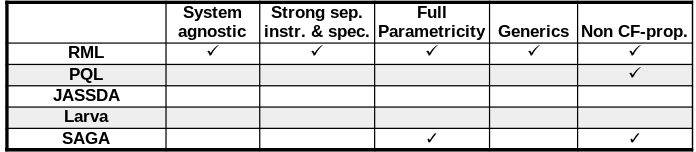
\includegraphics[width=0.6\textwidth,keepaspectratio=true]{tabella-viv3.jpg}[htb!]
%% \caption{Tools for RV of Java programs and their comparison with RML.}
%% \label{comparison}
%% \end{table*}


\bibliographystyle{ACM-Reference-Format}
\bibliography{biblio}

\appendix
\section{Example of verified Java code}\label{appendix}

A simple Java snippet verified by the \rml specification defined in \Cref{list:hash}.
\begin{lstlisting}[numbers=left]
var sset = new HashSet<Set<Integer>>();
var s1 = new HashSet<Integer>();
var s2 = new HashSet<Integer>();
s1.add(1);
s2.add(2);
sset.add(s1);
s1.contains(1);
s1.add(1);
sset.add(s2);
sset.remove(s1);
//s2.remove(2);
s1.remove(1);
s2.remove(1);
sset.remove(s2);
s1.add(1);
s2.add(2);
\end{lstlisting}
If line 11 is commented, then the code is correct w.r.t. the specification and the monitor successfully analyzes the whole trace generated by the execution of the snippet, consisting of 82 events stored in a log file:
\begin{lstlisting}[language={},basicstyle=\ttfamily\scriptsize]
...
matched event #82: _21156{argIds:[null],args:[2],event:func_post,name:add,res:false,targetId:13}
Execution terminated correctly
\end{lstlisting}

If line 11 is uncommented, then the code is not correct w.r.t. the specification because set \lstinline{s2} while
contained in the hash set \lstinline{sset}.

The monitor reports an error for event number 58 corresponding to the return from method call
at line 11, where 13 is the id of the object referenced by \lstinline{s2}:
\begin{lstlisting}[language={},basicstyle=\ttfamily\scriptsize]
unmatched event #58:
  _36564{argIds:[null],args:[2],event:func_post,name:remove,
         res:true,targetId:13}
\end{lstlisting}

\end{document}
\endinput
%%
%% End of file `sample-sigconf.tex'.
